% Copyright 2025  Ed Bueler

\documentclass[10pt,hyperref]{beamer}

\mode<presentation>
{
  \usetheme{Madrid}

  \usecolortheme{beaver}

  \setbeamercovered{transparent}
  
  \setbeamerfont{frametitle}{size=\large}
}

\setbeamercolor*{block title}{bg=red!10}
\setbeamercolor*{block body}{bg=red!5}

\usepackage[english]{babel}
\usepackage[latin1]{inputenc}
\usepackage{times}
\usepackage[T1]{fontenc}
% Or whatever. Note that the encoding and the font should match. If T1
% does not look nice, try deleting the line with the fontenc.

\usepackage{empheq}
\usepackage{animate}
\usepackage{bm,xspace,verbatim,fancyvrb}
\usepackage{hyperref}

% If you wish to uncover everything in a step-wise fashion, uncomment
% the following command: 
%\beamerdefaultoverlayspecification{<+->}

\newcommand{\bb}{\mathbf{b}}
\newcommand{\bc}{\mathbf{c}}
\newcommand{\bbf}{\mathbf{f}}
\newcommand{\bg}{\mathbf{g}}
\newcommand{\br}{\mathbf{r}}
\newcommand{\bx}{\mathbf{x}}
\newcommand{\by}{\mathbf{y}}
\newcommand{\bv}{\mathbf{v}}
\newcommand{\bu}{\mathbf{u}}
\newcommand{\bw}{\mathbf{w}}

\newcommand{\grad}{\nabla}
\newcommand{\Grad}{\grad}
\newcommand{\Div}{\nabla\cdot}
\newcommand{\Curl}{\nabla\times}

\newcommand{\CC}{\mathbb{C}}
\newcommand{\RR}{\mathbb{R}}

\newcommand{\ddt}[1]{\ensuremath{\frac{\partial #1}{\partial t}}}
\newcommand{\ddx}[1]{\ensuremath{\frac{\partial #1}{\partial x}}}
\renewcommand{\t}[1]{\texttt{#1}}
\newcommand{\Matlab}{\textsc{Matlab}\xspace}
\newcommand{\Octave}{\textsc{Octave}\xspace}
%\newcommand{\MO}{\Matlab/\Octave}
\newcommand{\MO}{\Matlab}
\newcommand{\eps}{\epsilon}

\newcommand{\MS}{\alert{MAKE SURE}\xspace}

\newcommand{\exer}[2]{\medskip\noindent \textbf{#1.}\quad #2}

\newcommand{\mfile}[1]{
\VerbatimInput[frame=single,label=\fbox{\scriptsize \textsl{\,#1\,}},fontfamily=courier,fontsize=\scriptsize]{#1}
}

\newcommand{\mfiletiny}[1]{
\VerbatimInput[frame=single,label=\fbox{\scriptsize \textsl{\,#1\,}},fontfamily=courier,fontsize=\tiny]{#1}
}

\DefineVerbatimEnvironment{mVerb}{Verbatim}{numbersep=2mm,framerule=0.1mm,framesep=2mm,xleftmargin=4mm,fontsize=\small}


\AtBeginSection[]
{
  \begin{frame}<beamer>
    \frametitle{Outline}
    \tableofcontents[currentsection,hideallsubsections]
  \end{frame}
}

\title{Navier-Stokes solved with finite elements}

\subtitle{in Firedrake}

\author{Ed Bueler}

\institute{MATH 692 Fluids \& Solids Seminar}

\date{Spring 2025}

\begin{document}
\beamertemplatenavigationsymbolsempty

\begin{frame}
  \maketitle
\end{frame}


\begin{frame}{flow assumptions}

\begin{itemize}
\item all examples here are for domains $\Omega \subset \RR^2$
\item denote: $\bu=\bu(t,x,y)$ is velocity and $p=p(t,x,y)$ is pressure
\item assume density $\rho>0$ is constant; fluid is incompressible
\item assume constant dynamic viscosity: $\sigma = -p I + 2 \mu D\bu$ for constant $\mu>0$
\item body force, possibly: $\bbf = \rho \bg$
\item units: $[\bu]=\text{m}\,\text{s}^{-1}$, $[p]=\text{N}\,\text{m}^{-2}\,\text{s}^{-1}$, $[\rho]=\text{kg}\,\text{m}^{-3}$, $[\mu]=\text{kg}\,\text{m}^{-1}\,\text{s}^{-1}$
\end{itemize}
\end{frame}


\begin{frame}{the Navier-Stokes model}

\begin{itemize}
\item the Navier-Stokes equations are:
\begin{align*}
\rho\left(\bu_t + \bu \cdot \grad \bu\right) &= \mu \grad^2 \bu - \grad p + \rho \bg & &\text{conservation of momentum} \\
\Div \bu &= 0 & &\text{incompressibility (c.~of mass)}
\end{align*}
\end{itemize}
\end{frame}


\begin{frame}{flow past a cylinder 1}

\begin{itemize}
\item Nick provided formula for the potential flow past a cylinder \dots recall
\item from Navier-Stokes, derive by taking the viscosity $\mu$ to be very large:
	$$\mu |\grad^2 \bu| \gg \rho|\left(\bu_t + \bu \cdot \grad \bu\right)|,\, |\grad p|,\, \rho |\bg|$$
\item equations simplify:
\begin{align*}
0 &= \mu \grad^2 \bu & &\text{conservation of momentum} \\
\Div \bu &= 0 & &\text{incompressibility (c.~of mass)}
\end{align*}
\item but, $\grad^2 \bu = \grad\left(\Div \bu\right) - \Curl(\Curl \bu)$, so vorticity is zero ($\bm{\omega}=\Curl\bu=0$)
\end{itemize}
\end{frame}


\begin{frame}{flow past a cylinder 2}

\begin{itemize}
\item vorticity is zero ($\Curl\bu=0$) so there exists a potential $\bu = \grad \phi$
\item by incompressibility $\phi$ is harmonic:
	$$\grad^2 \phi = 0$$
\item assume far field velocity $\bu=(U_0,0)$, non-penetration and free slip on circle $r=a$
\item get by separation of variables:
	$$\phi(r,\theta) = U_0 \left(r + \frac{a^2}{r}\right) \cos(\theta) \hspace{2.3in}$$
\end{itemize}

\vspace{-19mm}
\hfill
\mbox{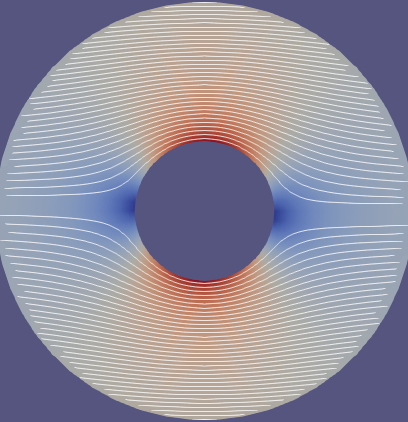
\includegraphics[width=0.37\textwidth]{figs/flowcyl.png} \qquad}
\end{frame}


\begin{frame}{}

\begin{itemize}
\item 
\end{itemize}
\end{frame}



\begin{frame}[fragile]{steepest-descent with back-tracking code}

\begin{itemize}
\item here is a basic implementation of \emph{steepest-descent} with \emph{back-tracking}
    \begin{itemize}
    \item[$=$] SDBT
    \end{itemize}
\item it assumes that the user supplies $x_0$ and a function $f$ that returns both the values $f(x)$ and the gradient $\grad f(x)$:

\medskip
\begin{Verbatim}[fontsize=\small]
function [z, xk, k] = sdbt(f, x0, tol)

xk = x0(:);
maxiters = 10000;
for k = 1:maxiters
    [fk, dfk] = f(xk);           % objective and gradient
    if norm(dfk) < tol
        z = fk;
        break                    % success
    end
    pk = - dfk(:);               % steepest descent
    alpha = bt(xk, pk, dfk, f);  % back-tracking
    xk = xk + alpha * pk;
end
\end{Verbatim}
\end{itemize}
\end{frame}





\begin{frame}{summary}

\begin{itemize}
\item steepest descent (gradient descent) simply uses the search direction $p_k = -\grad f(x_k)$
\item determining the step size $\alpha_k$, when actually taking the step, namely $x_{k+1}=x_k + \alpha_k p_k$, is nontrivial
    \begin{itemize}
    \item[$\circ$] line search (section 11.5) or trust region (11.6) is needed
    \item[$\circ$] for general functions, back-tracking is reasonable
    \item[$\circ$] for quadratic functions we can use the optimal step size
    \end{itemize}
\item even with good line search, steepest descent sucks
    \begin{itemize}
    \item[$\circ$] steepest descent is slow when contour lines (level sets) are highly curved

    \smallskip
    \item[$\circ$] going down the gradient is generally \alert{the wrong direction}:
        \begin{itemize}
        \item steepest descent direction $p_k = - I^{-1} \grad f(x_k)$ is wrong, while
        \item Newton direction $p_k = - (\grad^2f(x_k))^{-1} \grad f(x_k)$ is perfect for quadratic objectives
        \end{itemize}
    \item[$\circ$] the steepest-descent vector $p_k = -\grad f(x_k)$ has a length which depends on the scaling of $f(x)$, which is bad
        \begin{itemize}
        \item the Newton step does not have this flaw
        \end{itemize}
    \end{itemize}
\item however, functions like Rosenbrock remain difficult even for Newton
\end{itemize}
\end{frame}




\end{document}

